\documentclass[twoside]{book}

% Packages required by doxygen
\usepackage{fixltx2e}
\usepackage{calc}
\usepackage{doxygen}
\usepackage[export]{adjustbox} % also loads graphicx
\usepackage{graphicx}
\usepackage[utf8]{inputenc}
\usepackage{makeidx}
\usepackage{multicol}
\usepackage{multirow}
\PassOptionsToPackage{warn}{textcomp}
\usepackage{textcomp}
\usepackage[nointegrals]{wasysym}
\usepackage[table]{xcolor}

% Font selection
\usepackage[T1]{fontenc}
\usepackage[scaled=.90]{helvet}
\usepackage{courier}
\usepackage{amssymb}
\usepackage{sectsty}
\renewcommand{\familydefault}{\sfdefault}
\allsectionsfont{%
  \fontseries{bc}\selectfont%
  \color{darkgray}%
}
\renewcommand{\DoxyLabelFont}{%
  \fontseries{bc}\selectfont%
  \color{darkgray}%
}
\newcommand{\+}{\discretionary{\mbox{\scriptsize$\hookleftarrow$}}{}{}}

% Page & text layout
\usepackage{geometry}
\geometry{%
  a4paper,%
  top=2.5cm,%
  bottom=2.5cm,%
  left=2.5cm,%
  right=2.5cm%
}
\tolerance=750
\hfuzz=15pt
\hbadness=750
\setlength{\emergencystretch}{15pt}
\setlength{\parindent}{0cm}
\setlength{\parskip}{3ex plus 2ex minus 2ex}
\makeatletter
\renewcommand{\paragraph}{%
  \@startsection{paragraph}{4}{0ex}{-1.0ex}{1.0ex}{%
    \normalfont\normalsize\bfseries\SS@parafont%
  }%
}
\renewcommand{\subparagraph}{%
  \@startsection{subparagraph}{5}{0ex}{-1.0ex}{1.0ex}{%
    \normalfont\normalsize\bfseries\SS@subparafont%
  }%
}
\makeatother

% Headers & footers
\usepackage{fancyhdr}
\pagestyle{fancyplain}
\fancyhead[LE]{\fancyplain{}{\bfseries\thepage}}
\fancyhead[CE]{\fancyplain{}{}}
\fancyhead[RE]{\fancyplain{}{\bfseries\leftmark}}
\fancyhead[LO]{\fancyplain{}{\bfseries\rightmark}}
\fancyhead[CO]{\fancyplain{}{}}
\fancyhead[RO]{\fancyplain{}{\bfseries\thepage}}
\fancyfoot[LE]{\fancyplain{}{}}
\fancyfoot[CE]{\fancyplain{}{}}
\fancyfoot[RE]{\fancyplain{}{\bfseries\scriptsize Generated by Doxygen }}
\fancyfoot[LO]{\fancyplain{}{\bfseries\scriptsize Generated by Doxygen }}
\fancyfoot[CO]{\fancyplain{}{}}
\fancyfoot[RO]{\fancyplain{}{}}
\renewcommand{\footrulewidth}{0.4pt}
\renewcommand{\chaptermark}[1]{%
  \markboth{#1}{}%
}
\renewcommand{\sectionmark}[1]{%
  \markright{\thesection\ #1}%
}

% Indices & bibliography
\usepackage{natbib}
\usepackage[titles]{tocloft}
\setcounter{tocdepth}{3}
\setcounter{secnumdepth}{5}
\makeindex

% Hyperlinks (required, but should be loaded last)
\usepackage{ifpdf}
\ifpdf
  \usepackage[pdftex,pagebackref=true]{hyperref}
\else
  \usepackage[ps2pdf,pagebackref=true]{hyperref}
\fi
\hypersetup{%
  colorlinks=true,%
  linkcolor=blue,%
  citecolor=blue,%
  unicode%
}

% Custom commands
\newcommand{\clearemptydoublepage}{%
  \newpage{\pagestyle{empty}\cleardoublepage}%
}

\usepackage{caption}
\captionsetup{labelsep=space,justification=centering,font={bf},singlelinecheck=off,skip=4pt,position=top}

%===== C O N T E N T S =====

\begin{document}

% Titlepage & ToC
\hypersetup{pageanchor=false,
             bookmarksnumbered=true,
             pdfencoding=unicode
            }
\pagenumbering{alph}
\begin{titlepage}
\vspace*{7cm}
\begin{center}%
{\Large 3-\/uzd }\\
\vspace*{1cm}
{\large Generated by Doxygen 1.8.14}\\
\end{center}
\end{titlepage}
\clearemptydoublepage
\pagenumbering{roman}
\tableofcontents
\clearemptydoublepage
\pagenumbering{arabic}
\hypersetup{pageanchor=true}

%--- Begin generated contents ---
\chapter{Hierarchical Index}
\section{Class Hierarchy}
This inheritance list is sorted roughly, but not completely, alphabetically\+:\begin{DoxyCompactList}
\item \contentsline{section}{Person}{\pageref{classPerson}}{}
\begin{DoxyCompactList}
\item \contentsline{section}{Student}{\pageref{classStudent}}{}
\end{DoxyCompactList}
\end{DoxyCompactList}

\chapter{Class Index}
\section{Class List}
Here are the classes, structs, unions and interfaces with brief descriptions\+:\begin{DoxyCompactList}
\item\contentsline{section}{\mbox{\hyperlink{classPerson}{Person}} }{\pageref{classPerson}}{}
\item\contentsline{section}{\mbox{\hyperlink{classStudent}{Student}} }{\pageref{classStudent}}{}
\end{DoxyCompactList}

\chapter{File Index}
\section{File List}
Here is a list of all files with brief descriptions\+:\begin{DoxyCompactList}
\item\contentsline{section}{\mbox{\hyperlink{funkc_8cpp}{funkc.\+cpp}} }{\pageref{funkc_8cpp}}{}
\item\contentsline{section}{\mbox{\hyperlink{funkc_8h}{funkc.\+h}} }{\pageref{funkc_8h}}{}
\item\contentsline{section}{\mbox{\hyperlink{main_8cpp}{main.\+cpp}} }{\pageref{main_8cpp}}{}
\item\contentsline{section}{\mbox{\hyperlink{zmogus__studentas_8cpp}{zmogus\+\_\+studentas.\+cpp}} }{\pageref{zmogus__studentas_8cpp}}{}
\item\contentsline{section}{\mbox{\hyperlink{zmogus__studentas_8cpp_8h}{zmogus\+\_\+studentas.\+cpp.\+h}} }{\pageref{zmogus__studentas_8cpp_8h}}{}
\item\contentsline{section}{\mbox{\hyperlink{zmogus__studentas_8h}{zmogus\+\_\+studentas.\+h}} }{\pageref{zmogus__studentas_8h}}{}
\end{DoxyCompactList}

\chapter{Class Documentation}
\hypertarget{classPerson}{}\section{Person}
\label{classPerson}\index{Person@{Person}}


{\ttfamily \#include \char`\"{}zmogus\+\_\+studentas.\+h\char`\"{}}

Inheritance diagram for Person\+:\begin{figure}[H]
\begin{center}
\leavevmode
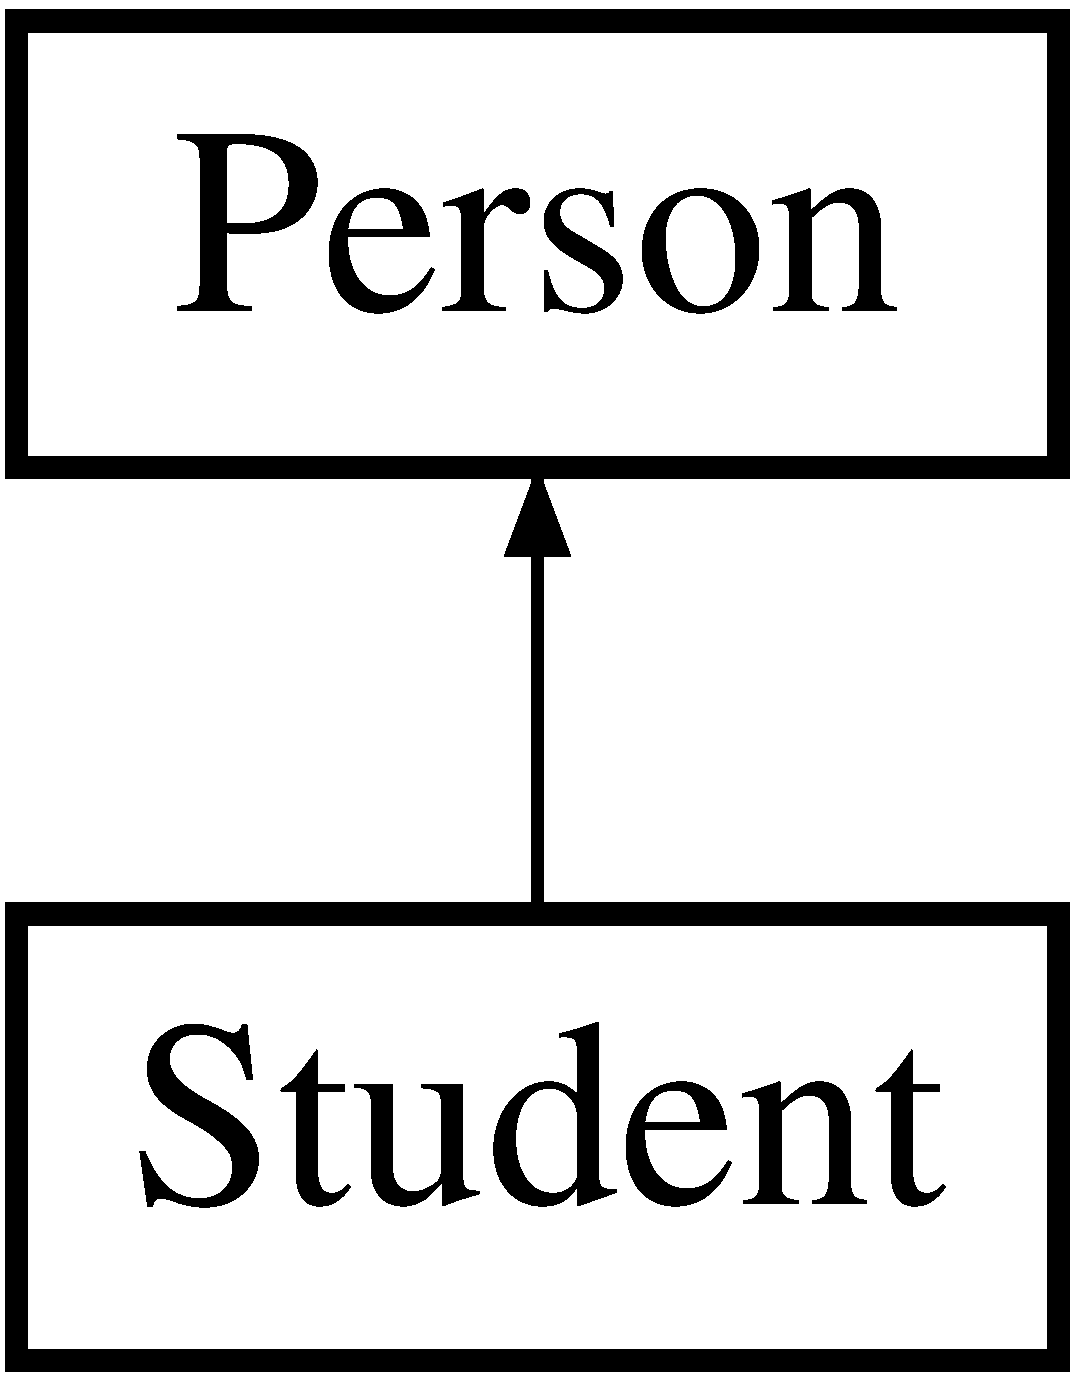
\includegraphics[height=2.000000cm]{classPerson}
\end{center}
\end{figure}
\subsection*{Public Member Functions}
\begin{DoxyCompactItemize}
\item 
string \mbox{\hyperlink{classPerson_ad2784fa1040db0a5123721226039c2c8}{get\+\_\+name}} () const
\item 
string \mbox{\hyperlink{classPerson_a2dfd43e34424a3c6f40598a6dc0b5f28}{get\+\_\+surname}} () const
\item 
void \mbox{\hyperlink{classPerson_abe323fe4507bbf06e7677cc049d9fa86}{set\+\_\+name}} (string t)
\item 
void \mbox{\hyperlink{classPerson_a7856672997420904aa1650806c6b2063}{set\+\_\+surname}} (string t)
\end{DoxyCompactItemize}
\subsection*{Protected Attributes}
\begin{DoxyCompactItemize}
\item 
string \mbox{\hyperlink{classPerson_a8ccf841cb59e451791bcb2e1ac4f1edc}{name}}
\item 
string \mbox{\hyperlink{classPerson_acb03bac0d1d003c3c1a88da1524d2c3a}{surname}}
\end{DoxyCompactItemize}


\subsection{Member Function Documentation}
\mbox{\Hypertarget{classPerson_ad2784fa1040db0a5123721226039c2c8}\label{classPerson_ad2784fa1040db0a5123721226039c2c8}} 
\index{Person@{Person}!get\+\_\+name@{get\+\_\+name}}
\index{get\+\_\+name@{get\+\_\+name}!Person@{Person}}
\subsubsection{\texorpdfstring{get\+\_\+name()}{get\_name()}}
{\footnotesize\ttfamily string get\+\_\+name (\begin{DoxyParamCaption}{ }\end{DoxyParamCaption}) const\hspace{0.3cm}{\ttfamily [inline]}}

\mbox{\Hypertarget{classPerson_a2dfd43e34424a3c6f40598a6dc0b5f28}\label{classPerson_a2dfd43e34424a3c6f40598a6dc0b5f28}} 
\index{Person@{Person}!get\+\_\+surname@{get\+\_\+surname}}
\index{get\+\_\+surname@{get\+\_\+surname}!Person@{Person}}
\subsubsection{\texorpdfstring{get\+\_\+surname()}{get\_surname()}}
{\footnotesize\ttfamily string get\+\_\+surname (\begin{DoxyParamCaption}{ }\end{DoxyParamCaption}) const\hspace{0.3cm}{\ttfamily [inline]}}

\mbox{\Hypertarget{classPerson_abe323fe4507bbf06e7677cc049d9fa86}\label{classPerson_abe323fe4507bbf06e7677cc049d9fa86}} 
\index{Person@{Person}!set\+\_\+name@{set\+\_\+name}}
\index{set\+\_\+name@{set\+\_\+name}!Person@{Person}}
\subsubsection{\texorpdfstring{set\+\_\+name()}{set\_name()}}
{\footnotesize\ttfamily void set\+\_\+name (\begin{DoxyParamCaption}\item[{string}]{t }\end{DoxyParamCaption})\hspace{0.3cm}{\ttfamily [inline]}}

\mbox{\Hypertarget{classPerson_a7856672997420904aa1650806c6b2063}\label{classPerson_a7856672997420904aa1650806c6b2063}} 
\index{Person@{Person}!set\+\_\+surname@{set\+\_\+surname}}
\index{set\+\_\+surname@{set\+\_\+surname}!Person@{Person}}
\subsubsection{\texorpdfstring{set\+\_\+surname()}{set\_surname()}}
{\footnotesize\ttfamily void set\+\_\+surname (\begin{DoxyParamCaption}\item[{string}]{t }\end{DoxyParamCaption})\hspace{0.3cm}{\ttfamily [inline]}}



\subsection{Member Data Documentation}
\mbox{\Hypertarget{classPerson_a8ccf841cb59e451791bcb2e1ac4f1edc}\label{classPerson_a8ccf841cb59e451791bcb2e1ac4f1edc}} 
\index{Person@{Person}!name@{name}}
\index{name@{name}!Person@{Person}}
\subsubsection{\texorpdfstring{name}{name}}
{\footnotesize\ttfamily string name\hspace{0.3cm}{\ttfamily [protected]}}

\mbox{\Hypertarget{classPerson_acb03bac0d1d003c3c1a88da1524d2c3a}\label{classPerson_acb03bac0d1d003c3c1a88da1524d2c3a}} 
\index{Person@{Person}!surname@{surname}}
\index{surname@{surname}!Person@{Person}}
\subsubsection{\texorpdfstring{surname}{surname}}
{\footnotesize\ttfamily string surname\hspace{0.3cm}{\ttfamily [protected]}}



The documentation for this class was generated from the following file\+:\begin{DoxyCompactItemize}
\item 
\mbox{\hyperlink{zmogus__studentas_8h}{zmogus\+\_\+studentas.\+h}}\end{DoxyCompactItemize}

\hypertarget{classStudent}{}\section{Student}
\label{classStudent}\index{Student@{Student}}


{\ttfamily \#include \char`\"{}zmogus\+\_\+studentas.\+h\char`\"{}}

Inheritance diagram for Student\+:\begin{figure}[H]
\begin{center}
\leavevmode
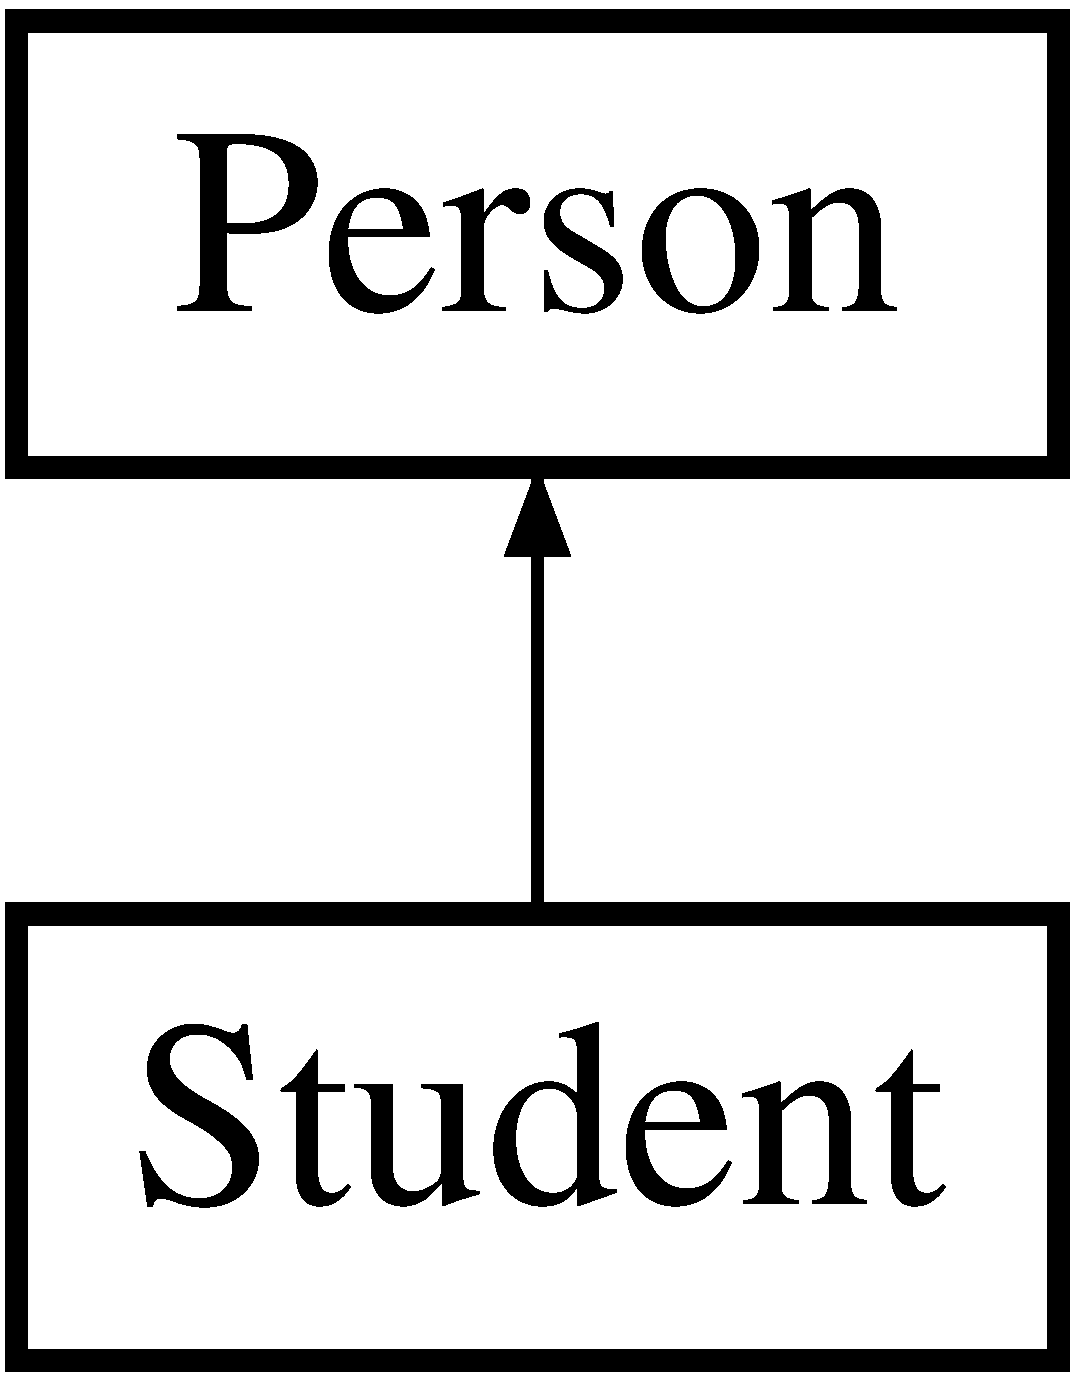
\includegraphics[height=2.000000cm]{classStudent}
\end{center}
\end{figure}
\subsection*{Public Member Functions}
\begin{DoxyCompactItemize}
\item 
\mbox{\hyperlink{classStudent_a26ceb532f001722145707442f5f26480}{Student}} ()
\item 
double \mbox{\hyperlink{classStudent_a6d3f7cc8886fe956a5de14b07e1ca457}{avg}} ()
\item 
double \mbox{\hyperlink{classStudent_ae99a413149615469071dc30895d34bca}{final\+\_\+mark}} ()
\item 
double \mbox{\hyperlink{classStudent_ab996e975f082192a02077a8c5665aa25}{get\+\_\+exam\+Mark}} ()
\item 
double \mbox{\hyperlink{classStudent_a227227aa7b579cc83a3e0d37bd309e59}{get\+\_\+final\+Mark}} ()
\item 
int \mbox{\hyperlink{classStudent_a94ee4d5b4ddd8e4b2ac5204453fb1f6d}{get\+\_\+mark}} (int i)
\item 
bool \mbox{\hyperlink{classStudent_ab1f4cbc4e32a29b489b87b31366bb4e7}{operator!=}} (\mbox{\hyperlink{classStudent}{Student}} \&a)
\item 
bool \mbox{\hyperlink{classStudent_aac01d66b5c4cf429210264eb9d33c84e}{operator$<$}} (\mbox{\hyperlink{classStudent}{Student}} \&a)
\item 
bool \mbox{\hyperlink{classStudent_af3677abbb99886c6c422c63ed2967c19}{operator==}} (\mbox{\hyperlink{classStudent}{Student}} \&a)
\item 
bool \mbox{\hyperlink{classStudent_aa0d55242e485d234a9df02cc1065bc94}{operator$>$}} (\mbox{\hyperlink{classStudent}{Student}} \&a)
\item 
void \mbox{\hyperlink{classStudent_a51de6f509d2414a9cc9ddae1198f020c}{set\+\_\+exam\+Mark}} (int m)
\item 
void \mbox{\hyperlink{classStudent_a08cede177ec5ed67bec7281eaced7b8e}{set\+\_\+mark}} (int m)
\end{DoxyCompactItemize}
\subsection*{Protected Attributes}
\begin{DoxyCompactItemize}
\item 
double \mbox{\hyperlink{classStudent_a6b1356b600cbdfe6928d5f020bc35233}{exam\+Mark}}
\item 
double \mbox{\hyperlink{classStudent_ae4f6dc231d21f3ae7386114d1b572cf0}{final\+Mark}}
\item 
vector$<$ int $>$ \mbox{\hyperlink{classStudent_a460302cb4e9860802f65d94255a93811}{marks}}
\end{DoxyCompactItemize}


\subsection{Constructor \& Destructor Documentation}
\mbox{\Hypertarget{classStudent_a26ceb532f001722145707442f5f26480}\label{classStudent_a26ceb532f001722145707442f5f26480}} 
\index{Student@{Student}!Student@{Student}}
\index{Student@{Student}!Student@{Student}}
\subsubsection{\texorpdfstring{Student()}{Student()}}
{\footnotesize\ttfamily \mbox{\hyperlink{classStudent}{Student}} (\begin{DoxyParamCaption}{ }\end{DoxyParamCaption})\hspace{0.3cm}{\ttfamily [inline]}}



\subsection{Member Function Documentation}
\mbox{\Hypertarget{classStudent_a6d3f7cc8886fe956a5de14b07e1ca457}\label{classStudent_a6d3f7cc8886fe956a5de14b07e1ca457}} 
\index{Student@{Student}!avg@{avg}}
\index{avg@{avg}!Student@{Student}}
\subsubsection{\texorpdfstring{avg()}{avg()}}
{\footnotesize\ttfamily double avg (\begin{DoxyParamCaption}{ }\end{DoxyParamCaption})}

\mbox{\Hypertarget{classStudent_ae99a413149615469071dc30895d34bca}\label{classStudent_ae99a413149615469071dc30895d34bca}} 
\index{Student@{Student}!final\+\_\+mark@{final\+\_\+mark}}
\index{final\+\_\+mark@{final\+\_\+mark}!Student@{Student}}
\subsubsection{\texorpdfstring{final\+\_\+mark()}{final\_mark()}}
{\footnotesize\ttfamily double final\+\_\+mark (\begin{DoxyParamCaption}{ }\end{DoxyParamCaption})}

\mbox{\Hypertarget{classStudent_ab996e975f082192a02077a8c5665aa25}\label{classStudent_ab996e975f082192a02077a8c5665aa25}} 
\index{Student@{Student}!get\+\_\+exam\+Mark@{get\+\_\+exam\+Mark}}
\index{get\+\_\+exam\+Mark@{get\+\_\+exam\+Mark}!Student@{Student}}
\subsubsection{\texorpdfstring{get\+\_\+exam\+Mark()}{get\_examMark()}}
{\footnotesize\ttfamily double get\+\_\+exam\+Mark (\begin{DoxyParamCaption}{ }\end{DoxyParamCaption})\hspace{0.3cm}{\ttfamily [inline]}}

\mbox{\Hypertarget{classStudent_a227227aa7b579cc83a3e0d37bd309e59}\label{classStudent_a227227aa7b579cc83a3e0d37bd309e59}} 
\index{Student@{Student}!get\+\_\+final\+Mark@{get\+\_\+final\+Mark}}
\index{get\+\_\+final\+Mark@{get\+\_\+final\+Mark}!Student@{Student}}
\subsubsection{\texorpdfstring{get\+\_\+final\+Mark()}{get\_finalMark()}}
{\footnotesize\ttfamily double get\+\_\+final\+Mark (\begin{DoxyParamCaption}{ }\end{DoxyParamCaption})\hspace{0.3cm}{\ttfamily [inline]}}

\mbox{\Hypertarget{classStudent_a94ee4d5b4ddd8e4b2ac5204453fb1f6d}\label{classStudent_a94ee4d5b4ddd8e4b2ac5204453fb1f6d}} 
\index{Student@{Student}!get\+\_\+mark@{get\+\_\+mark}}
\index{get\+\_\+mark@{get\+\_\+mark}!Student@{Student}}
\subsubsection{\texorpdfstring{get\+\_\+mark()}{get\_mark()}}
{\footnotesize\ttfamily int get\+\_\+mark (\begin{DoxyParamCaption}\item[{int}]{i }\end{DoxyParamCaption})\hspace{0.3cm}{\ttfamily [inline]}}

\mbox{\Hypertarget{classStudent_ab1f4cbc4e32a29b489b87b31366bb4e7}\label{classStudent_ab1f4cbc4e32a29b489b87b31366bb4e7}} 
\index{Student@{Student}!operator"!=@{operator"!=}}
\index{operator"!=@{operator"!=}!Student@{Student}}
\subsubsection{\texorpdfstring{operator"!=()}{operator!=()}}
{\footnotesize\ttfamily bool operator!= (\begin{DoxyParamCaption}\item[{\mbox{\hyperlink{classStudent}{Student}} \&}]{a }\end{DoxyParamCaption})}

\mbox{\Hypertarget{classStudent_aac01d66b5c4cf429210264eb9d33c84e}\label{classStudent_aac01d66b5c4cf429210264eb9d33c84e}} 
\index{Student@{Student}!operator$<$@{operator$<$}}
\index{operator$<$@{operator$<$}!Student@{Student}}
\subsubsection{\texorpdfstring{operator$<$()}{operator<()}}
{\footnotesize\ttfamily bool operator$<$ (\begin{DoxyParamCaption}\item[{\mbox{\hyperlink{classStudent}{Student}} \&}]{a }\end{DoxyParamCaption})}

\mbox{\Hypertarget{classStudent_af3677abbb99886c6c422c63ed2967c19}\label{classStudent_af3677abbb99886c6c422c63ed2967c19}} 
\index{Student@{Student}!operator==@{operator==}}
\index{operator==@{operator==}!Student@{Student}}
\subsubsection{\texorpdfstring{operator==()}{operator==()}}
{\footnotesize\ttfamily bool operator== (\begin{DoxyParamCaption}\item[{\mbox{\hyperlink{classStudent}{Student}} \&}]{a }\end{DoxyParamCaption})}

\mbox{\Hypertarget{classStudent_aa0d55242e485d234a9df02cc1065bc94}\label{classStudent_aa0d55242e485d234a9df02cc1065bc94}} 
\index{Student@{Student}!operator$>$@{operator$>$}}
\index{operator$>$@{operator$>$}!Student@{Student}}
\subsubsection{\texorpdfstring{operator$>$()}{operator>()}}
{\footnotesize\ttfamily bool operator$>$ (\begin{DoxyParamCaption}\item[{\mbox{\hyperlink{classStudent}{Student}} \&}]{a }\end{DoxyParamCaption})}

\mbox{\Hypertarget{classStudent_a51de6f509d2414a9cc9ddae1198f020c}\label{classStudent_a51de6f509d2414a9cc9ddae1198f020c}} 
\index{Student@{Student}!set\+\_\+exam\+Mark@{set\+\_\+exam\+Mark}}
\index{set\+\_\+exam\+Mark@{set\+\_\+exam\+Mark}!Student@{Student}}
\subsubsection{\texorpdfstring{set\+\_\+exam\+Mark()}{set\_examMark()}}
{\footnotesize\ttfamily void set\+\_\+exam\+Mark (\begin{DoxyParamCaption}\item[{int}]{m }\end{DoxyParamCaption})\hspace{0.3cm}{\ttfamily [inline]}}

\mbox{\Hypertarget{classStudent_a08cede177ec5ed67bec7281eaced7b8e}\label{classStudent_a08cede177ec5ed67bec7281eaced7b8e}} 
\index{Student@{Student}!set\+\_\+mark@{set\+\_\+mark}}
\index{set\+\_\+mark@{set\+\_\+mark}!Student@{Student}}
\subsubsection{\texorpdfstring{set\+\_\+mark()}{set\_mark()}}
{\footnotesize\ttfamily void set\+\_\+mark (\begin{DoxyParamCaption}\item[{int}]{m }\end{DoxyParamCaption})\hspace{0.3cm}{\ttfamily [inline]}}



\subsection{Member Data Documentation}
\mbox{\Hypertarget{classStudent_a6b1356b600cbdfe6928d5f020bc35233}\label{classStudent_a6b1356b600cbdfe6928d5f020bc35233}} 
\index{Student@{Student}!exam\+Mark@{exam\+Mark}}
\index{exam\+Mark@{exam\+Mark}!Student@{Student}}
\subsubsection{\texorpdfstring{exam\+Mark}{examMark}}
{\footnotesize\ttfamily double exam\+Mark\hspace{0.3cm}{\ttfamily [protected]}}

\mbox{\Hypertarget{classStudent_ae4f6dc231d21f3ae7386114d1b572cf0}\label{classStudent_ae4f6dc231d21f3ae7386114d1b572cf0}} 
\index{Student@{Student}!final\+Mark@{final\+Mark}}
\index{final\+Mark@{final\+Mark}!Student@{Student}}
\subsubsection{\texorpdfstring{final\+Mark}{finalMark}}
{\footnotesize\ttfamily double final\+Mark\hspace{0.3cm}{\ttfamily [protected]}}

\mbox{\Hypertarget{classStudent_a460302cb4e9860802f65d94255a93811}\label{classStudent_a460302cb4e9860802f65d94255a93811}} 
\index{Student@{Student}!marks@{marks}}
\index{marks@{marks}!Student@{Student}}
\subsubsection{\texorpdfstring{marks}{marks}}
{\footnotesize\ttfamily vector$<$int$>$ marks\hspace{0.3cm}{\ttfamily [protected]}}



The documentation for this class was generated from the following files\+:\begin{DoxyCompactItemize}
\item 
\mbox{\hyperlink{zmogus__studentas_8h}{zmogus\+\_\+studentas.\+h}}\item 
\mbox{\hyperlink{zmogus__studentas_8cpp}{zmogus\+\_\+studentas.\+cpp}}\end{DoxyCompactItemize}

\chapter{File Documentation}
\hypertarget{funkc_8cpp}{}\section{funkc.\+cpp File Reference}
\label{funkc_8cpp}\index{funkc.\+cpp@{funkc.\+cpp}}
{\ttfamily \#include $<$iostream$>$}\newline
{\ttfamily \#include $<$iomanip$>$}\newline
{\ttfamily \#include $<$fstream$>$}\newline
{\ttfamily \#include $<$random$>$}\newline
{\ttfamily \#include $<$chrono$>$}\newline
{\ttfamily \#include $<$sstream$>$}\newline
{\ttfamily \#include $<$vector$>$}\newline
{\ttfamily \#include $<$cmath$>$}\newline
{\ttfamily \#include \char`\"{}funkc.\+h\char`\"{}}\newline
{\ttfamily \#include \char`\"{}zmogus\+\_\+studentas.\+h\char`\"{}}\newline
\subsection*{Macros}
\begin{DoxyCompactItemize}
\item 
\#define \mbox{\hyperlink{funkc_8cpp_a59afc168e06f175c818dd70436fa8cf0}{I\+N\+C\+\_\+3\+\_\+\+P\+E\+R\+\_\+\+N\+A\+U\+J\+A\+\_\+\+F\+U\+N\+K\+C\+\_\+H}}
\end{DoxyCompactItemize}
\subsection*{Functions}
\begin{DoxyCompactItemize}
\item 
void \mbox{\hyperlink{funkc_8cpp_aceb6740c86582bda5afc4812fc92eeb2}{file\+Read}} (vector$<$ \mbox{\hyperlink{classStudent}{Student}} $>$ \&\mbox{\hyperlink{funkc_8h_afbfeccb5b885c0a4659c5b44a7bbb856}{stud}})
\item 
void \mbox{\hyperlink{funkc_8cpp_ab4055b1ee4a3581dff8f6c8cb0158726}{file\+Write}} (int t, string file\+Name)
\item 
void \mbox{\hyperlink{funkc_8cpp_a38f6918b346b5f94ba6d067f8bf0cb25}{file\+Write\+Res}} (vector$<$ \mbox{\hyperlink{classStudent}{Student}} $>$ \mbox{\hyperlink{funkc_8h_afbfeccb5b885c0a4659c5b44a7bbb856}{stud}}, string file\+Name)
\item 
void \mbox{\hyperlink{funkc_8cpp_abfcda40e8fee1cb4726a7531d6a70865}{input}} (int \&num)
\item 
int \mbox{\hyperlink{funkc_8cpp_a0154314d58ed800336197efeb5b75e87}{random\+Mark}} ()
\end{DoxyCompactItemize}


\subsection{Macro Definition Documentation}
\mbox{\Hypertarget{funkc_8cpp_a59afc168e06f175c818dd70436fa8cf0}\label{funkc_8cpp_a59afc168e06f175c818dd70436fa8cf0}} 
\index{funkc.\+cpp@{funkc.\+cpp}!I\+N\+C\+\_\+3\+\_\+\+P\+E\+R\+\_\+\+N\+A\+U\+J\+A\+\_\+\+F\+U\+N\+K\+C\+\_\+H@{I\+N\+C\+\_\+3\+\_\+\+P\+E\+R\+\_\+\+N\+A\+U\+J\+A\+\_\+\+F\+U\+N\+K\+C\+\_\+H}}
\index{I\+N\+C\+\_\+3\+\_\+\+P\+E\+R\+\_\+\+N\+A\+U\+J\+A\+\_\+\+F\+U\+N\+K\+C\+\_\+H@{I\+N\+C\+\_\+3\+\_\+\+P\+E\+R\+\_\+\+N\+A\+U\+J\+A\+\_\+\+F\+U\+N\+K\+C\+\_\+H}!funkc.\+cpp@{funkc.\+cpp}}
\subsubsection{\texorpdfstring{I\+N\+C\+\_\+3\+\_\+\+P\+E\+R\+\_\+\+N\+A\+U\+J\+A\+\_\+\+F\+U\+N\+K\+C\+\_\+H}{INC\_3\_PER\_NAUJA\_FUNKC\_H}}
{\footnotesize\ttfamily \#define I\+N\+C\+\_\+3\+\_\+\+P\+E\+R\+\_\+\+N\+A\+U\+J\+A\+\_\+\+F\+U\+N\+K\+C\+\_\+H}



\subsection{Function Documentation}
\mbox{\Hypertarget{funkc_8cpp_aceb6740c86582bda5afc4812fc92eeb2}\label{funkc_8cpp_aceb6740c86582bda5afc4812fc92eeb2}} 
\index{funkc.\+cpp@{funkc.\+cpp}!file\+Read@{file\+Read}}
\index{file\+Read@{file\+Read}!funkc.\+cpp@{funkc.\+cpp}}
\subsubsection{\texorpdfstring{file\+Read()}{fileRead()}}
{\footnotesize\ttfamily void file\+Read (\begin{DoxyParamCaption}\item[{vector$<$ \mbox{\hyperlink{classStudent}{Student}} $>$ \&}]{stud }\end{DoxyParamCaption})}

\mbox{\Hypertarget{funkc_8cpp_ab4055b1ee4a3581dff8f6c8cb0158726}\label{funkc_8cpp_ab4055b1ee4a3581dff8f6c8cb0158726}} 
\index{funkc.\+cpp@{funkc.\+cpp}!file\+Write@{file\+Write}}
\index{file\+Write@{file\+Write}!funkc.\+cpp@{funkc.\+cpp}}
\subsubsection{\texorpdfstring{file\+Write()}{fileWrite()}}
{\footnotesize\ttfamily void file\+Write (\begin{DoxyParamCaption}\item[{int}]{t,  }\item[{string}]{file\+Name }\end{DoxyParamCaption})}

\mbox{\Hypertarget{funkc_8cpp_a38f6918b346b5f94ba6d067f8bf0cb25}\label{funkc_8cpp_a38f6918b346b5f94ba6d067f8bf0cb25}} 
\index{funkc.\+cpp@{funkc.\+cpp}!file\+Write\+Res@{file\+Write\+Res}}
\index{file\+Write\+Res@{file\+Write\+Res}!funkc.\+cpp@{funkc.\+cpp}}
\subsubsection{\texorpdfstring{file\+Write\+Res()}{fileWriteRes()}}
{\footnotesize\ttfamily void file\+Write\+Res (\begin{DoxyParamCaption}\item[{vector$<$ \mbox{\hyperlink{classStudent}{Student}} $>$}]{stud,  }\item[{string}]{file\+Name }\end{DoxyParamCaption})}

\mbox{\Hypertarget{funkc_8cpp_abfcda40e8fee1cb4726a7531d6a70865}\label{funkc_8cpp_abfcda40e8fee1cb4726a7531d6a70865}} 
\index{funkc.\+cpp@{funkc.\+cpp}!input@{input}}
\index{input@{input}!funkc.\+cpp@{funkc.\+cpp}}
\subsubsection{\texorpdfstring{input()}{input()}}
{\footnotesize\ttfamily void input (\begin{DoxyParamCaption}\item[{int \&}]{num }\end{DoxyParamCaption})}

\mbox{\Hypertarget{funkc_8cpp_a0154314d58ed800336197efeb5b75e87}\label{funkc_8cpp_a0154314d58ed800336197efeb5b75e87}} 
\index{funkc.\+cpp@{funkc.\+cpp}!random\+Mark@{random\+Mark}}
\index{random\+Mark@{random\+Mark}!funkc.\+cpp@{funkc.\+cpp}}
\subsubsection{\texorpdfstring{random\+Mark()}{randomMark()}}
{\footnotesize\ttfamily int random\+Mark (\begin{DoxyParamCaption}{ }\end{DoxyParamCaption})}


\hypertarget{funkc_8h}{}\section{funkc.\+h File Reference}
\label{funkc_8h}\index{funkc.\+h@{funkc.\+h}}
{\ttfamily \#include $<$iostream$>$}\newline
{\ttfamily \#include $<$iomanip$>$}\newline
{\ttfamily \#include $<$fstream$>$}\newline
{\ttfamily \#include $<$random$>$}\newline
{\ttfamily \#include $<$chrono$>$}\newline
{\ttfamily \#include $<$sstream$>$}\newline
{\ttfamily \#include $<$vector$>$}\newline
{\ttfamily \#include $<$cmath$>$}\newline
{\ttfamily \#include $<$functional$>$}\newline
{\ttfamily \#include \char`\"{}zmogus\+\_\+studentas.\+h\char`\"{}}\newline
\subsection*{Functions}
\begin{DoxyCompactItemize}
\item 
void \mbox{\hyperlink{funkc_8h_ac0a51e50a3a37ebbd5a5d6df3bff5b61}{file\+Read}} ()
\item 
void \mbox{\hyperlink{funkc_8h_a48d87b79477a44c2176d07762b78faaf}{file\+Write}} (int t)
\item 
int \mbox{\hyperlink{funkc_8h_a0154314d58ed800336197efeb5b75e87}{random\+Mark}} ()
\end{DoxyCompactItemize}
\subsection*{Variables}
\begin{DoxyCompactItemize}
\item 
vector$<$ \mbox{\hyperlink{classStudent}{Student}} $>$ \mbox{\hyperlink{funkc_8h_afbfeccb5b885c0a4659c5b44a7bbb856}{stud}}
\end{DoxyCompactItemize}


\subsection{Function Documentation}
\mbox{\Hypertarget{funkc_8h_ac0a51e50a3a37ebbd5a5d6df3bff5b61}\label{funkc_8h_ac0a51e50a3a37ebbd5a5d6df3bff5b61}} 
\index{funkc.\+h@{funkc.\+h}!file\+Read@{file\+Read}}
\index{file\+Read@{file\+Read}!funkc.\+h@{funkc.\+h}}
\subsubsection{\texorpdfstring{file\+Read()}{fileRead()}}
{\footnotesize\ttfamily void file\+Read (\begin{DoxyParamCaption}{ }\end{DoxyParamCaption})}

\mbox{\Hypertarget{funkc_8h_a48d87b79477a44c2176d07762b78faaf}\label{funkc_8h_a48d87b79477a44c2176d07762b78faaf}} 
\index{funkc.\+h@{funkc.\+h}!file\+Write@{file\+Write}}
\index{file\+Write@{file\+Write}!funkc.\+h@{funkc.\+h}}
\subsubsection{\texorpdfstring{file\+Write()}{fileWrite()}}
{\footnotesize\ttfamily void file\+Write (\begin{DoxyParamCaption}\item[{int}]{t }\end{DoxyParamCaption})}

\mbox{\Hypertarget{funkc_8h_a0154314d58ed800336197efeb5b75e87}\label{funkc_8h_a0154314d58ed800336197efeb5b75e87}} 
\index{funkc.\+h@{funkc.\+h}!random\+Mark@{random\+Mark}}
\index{random\+Mark@{random\+Mark}!funkc.\+h@{funkc.\+h}}
\subsubsection{\texorpdfstring{random\+Mark()}{randomMark()}}
{\footnotesize\ttfamily int random\+Mark (\begin{DoxyParamCaption}{ }\end{DoxyParamCaption})}



\subsection{Variable Documentation}
\mbox{\Hypertarget{funkc_8h_afbfeccb5b885c0a4659c5b44a7bbb856}\label{funkc_8h_afbfeccb5b885c0a4659c5b44a7bbb856}} 
\index{funkc.\+h@{funkc.\+h}!stud@{stud}}
\index{stud@{stud}!funkc.\+h@{funkc.\+h}}
\subsubsection{\texorpdfstring{stud}{stud}}
{\footnotesize\ttfamily vector$<$\mbox{\hyperlink{classStudent}{Student}}$>$ stud}


\hypertarget{main_8cpp}{}\section{main.\+cpp File Reference}
\label{main_8cpp}\index{main.\+cpp@{main.\+cpp}}
{\ttfamily \#include $<$iostream$>$}\newline
{\ttfamily \#include $<$algorithm$>$}\newline
{\ttfamily \#include $<$vector$>$}\newline
{\ttfamily \#include \char`\"{}zmogus\+\_\+studentas.\+h\char`\"{}}\newline
{\ttfamily \#include \char`\"{}funkc.\+h\char`\"{}}\newline
\subsection*{Functions}
\begin{DoxyCompactItemize}
\item 
int \mbox{\hyperlink{main_8cpp_ae66f6b31b5ad750f1fe042a706a4e3d4}{main}} ()
\end{DoxyCompactItemize}


\subsection{Function Documentation}
\mbox{\Hypertarget{main_8cpp_ae66f6b31b5ad750f1fe042a706a4e3d4}\label{main_8cpp_ae66f6b31b5ad750f1fe042a706a4e3d4}} 
\index{main.\+cpp@{main.\+cpp}!main@{main}}
\index{main@{main}!main.\+cpp@{main.\+cpp}}
\subsubsection{\texorpdfstring{main()}{main()}}
{\footnotesize\ttfamily int main (\begin{DoxyParamCaption}{ }\end{DoxyParamCaption})}


\hypertarget{zmogus__studentas_8cpp}{}\section{zmogus\+\_\+studentas.\+cpp File Reference}
\label{zmogus__studentas_8cpp}\index{zmogus\+\_\+studentas.\+cpp@{zmogus\+\_\+studentas.\+cpp}}
{\ttfamily \#include \char`\"{}zmogus\+\_\+studentas.\+h\char`\"{}}\newline
{\ttfamily \#include $<$iostream$>$}\newline
{\ttfamily \#include $<$algorithm$>$}\newline
{\ttfamily \#include $<$iomanip$>$}\newline
\subsection*{Functions}
\begin{DoxyCompactItemize}
\item 
bool \mbox{\hyperlink{zmogus__studentas_8cpp_ab7fca6938f3a35162fd5bce0cf91d80b}{is\+\_\+\+Loser}} (\mbox{\hyperlink{classStudent}{Student}} \&a)
\item 
bool \mbox{\hyperlink{zmogus__studentas_8cpp_a2a81cf36bb07349c3591fae7ec307e5e}{sort\+By\+Final}} (\mbox{\hyperlink{classStudent}{Student}} \&a, \mbox{\hyperlink{classStudent}{Student}} \&b)
\item 
bool \mbox{\hyperlink{zmogus__studentas_8cpp_ad9f64389db812f748880428737685f5b}{sort\+By\+Final\+Max\+To\+Min}} (\mbox{\hyperlink{classStudent}{Student}} \&a, \mbox{\hyperlink{classStudent}{Student}} \&b)
\item 
bool \mbox{\hyperlink{zmogus__studentas_8cpp_aba47559c3100ea6b38af4da0074434ed}{sort\+By\+Surname}} (\mbox{\hyperlink{classStudent}{Student}} \&a, \mbox{\hyperlink{classStudent}{Student}} \&b)
\end{DoxyCompactItemize}


\subsection{Function Documentation}
\mbox{\Hypertarget{zmogus__studentas_8cpp_ab7fca6938f3a35162fd5bce0cf91d80b}\label{zmogus__studentas_8cpp_ab7fca6938f3a35162fd5bce0cf91d80b}} 
\index{zmogus\+\_\+studentas.\+cpp@{zmogus\+\_\+studentas.\+cpp}!is\+\_\+\+Loser@{is\+\_\+\+Loser}}
\index{is\+\_\+\+Loser@{is\+\_\+\+Loser}!zmogus\+\_\+studentas.\+cpp@{zmogus\+\_\+studentas.\+cpp}}
\subsubsection{\texorpdfstring{is\+\_\+\+Loser()}{is\_Loser()}}
{\footnotesize\ttfamily bool is\+\_\+\+Loser (\begin{DoxyParamCaption}\item[{\mbox{\hyperlink{classStudent}{Student}} \&}]{a }\end{DoxyParamCaption})}

\mbox{\Hypertarget{zmogus__studentas_8cpp_a2a81cf36bb07349c3591fae7ec307e5e}\label{zmogus__studentas_8cpp_a2a81cf36bb07349c3591fae7ec307e5e}} 
\index{zmogus\+\_\+studentas.\+cpp@{zmogus\+\_\+studentas.\+cpp}!sort\+By\+Final@{sort\+By\+Final}}
\index{sort\+By\+Final@{sort\+By\+Final}!zmogus\+\_\+studentas.\+cpp@{zmogus\+\_\+studentas.\+cpp}}
\subsubsection{\texorpdfstring{sort\+By\+Final()}{sortByFinal()}}
{\footnotesize\ttfamily bool sort\+By\+Final (\begin{DoxyParamCaption}\item[{\mbox{\hyperlink{classStudent}{Student}} \&}]{a,  }\item[{\mbox{\hyperlink{classStudent}{Student}} \&}]{b }\end{DoxyParamCaption})}

\mbox{\Hypertarget{zmogus__studentas_8cpp_ad9f64389db812f748880428737685f5b}\label{zmogus__studentas_8cpp_ad9f64389db812f748880428737685f5b}} 
\index{zmogus\+\_\+studentas.\+cpp@{zmogus\+\_\+studentas.\+cpp}!sort\+By\+Final\+Max\+To\+Min@{sort\+By\+Final\+Max\+To\+Min}}
\index{sort\+By\+Final\+Max\+To\+Min@{sort\+By\+Final\+Max\+To\+Min}!zmogus\+\_\+studentas.\+cpp@{zmogus\+\_\+studentas.\+cpp}}
\subsubsection{\texorpdfstring{sort\+By\+Final\+Max\+To\+Min()}{sortByFinalMaxToMin()}}
{\footnotesize\ttfamily bool sort\+By\+Final\+Max\+To\+Min (\begin{DoxyParamCaption}\item[{\mbox{\hyperlink{classStudent}{Student}} \&}]{a,  }\item[{\mbox{\hyperlink{classStudent}{Student}} \&}]{b }\end{DoxyParamCaption})}

\mbox{\Hypertarget{zmogus__studentas_8cpp_aba47559c3100ea6b38af4da0074434ed}\label{zmogus__studentas_8cpp_aba47559c3100ea6b38af4da0074434ed}} 
\index{zmogus\+\_\+studentas.\+cpp@{zmogus\+\_\+studentas.\+cpp}!sort\+By\+Surname@{sort\+By\+Surname}}
\index{sort\+By\+Surname@{sort\+By\+Surname}!zmogus\+\_\+studentas.\+cpp@{zmogus\+\_\+studentas.\+cpp}}
\subsubsection{\texorpdfstring{sort\+By\+Surname()}{sortBySurname()}}
{\footnotesize\ttfamily bool sort\+By\+Surname (\begin{DoxyParamCaption}\item[{\mbox{\hyperlink{classStudent}{Student}} \&}]{a,  }\item[{\mbox{\hyperlink{classStudent}{Student}} \&}]{b }\end{DoxyParamCaption})}


\hypertarget{zmogus__studentas_8cpp_8h}{}\section{zmogus\+\_\+studentas.\+cpp.\+h File Reference}
\label{zmogus__studentas_8cpp_8h}\index{zmogus\+\_\+studentas.\+cpp.\+h@{zmogus\+\_\+studentas.\+cpp.\+h}}

\hypertarget{zmogus__studentas_8h}{}\section{zmogus\+\_\+studentas.\+h File Reference}
\label{zmogus__studentas_8h}\index{zmogus\+\_\+studentas.\+h@{zmogus\+\_\+studentas.\+h}}
{\ttfamily \#include $<$string$>$}\newline
{\ttfamily \#include $<$vector$>$}\newline
\subsection*{Classes}
\begin{DoxyCompactItemize}
\item 
class \mbox{\hyperlink{classPerson}{Person}}
\item 
class \mbox{\hyperlink{classStudent}{Student}}
\end{DoxyCompactItemize}
\subsection*{Functions}
\begin{DoxyCompactItemize}
\item 
void \mbox{\hyperlink{zmogus__studentas_8h_a7c5778e39957cb4da4884846c0e1f9f0}{file\+Read}} (vector$<$ \mbox{\hyperlink{classStudent}{Student}} $>$ \&)
\item 
void \mbox{\hyperlink{zmogus__studentas_8h_ab4055b1ee4a3581dff8f6c8cb0158726}{file\+Write}} (int t, string file\+Name)
\item 
void \mbox{\hyperlink{zmogus__studentas_8h_a0b7f093257f211ffde8a0644d3d70bff}{file\+Write\+Res}} (vector$<$ \mbox{\hyperlink{classStudent}{Student}} $>$, string file\+Name)
\item 
void \mbox{\hyperlink{zmogus__studentas_8h_abfcda40e8fee1cb4726a7531d6a70865}{input}} (int \&num)
\item 
bool \mbox{\hyperlink{zmogus__studentas_8h_ab7fca6938f3a35162fd5bce0cf91d80b}{is\+\_\+\+Loser}} (\mbox{\hyperlink{classStudent}{Student}} \&a)
\item 
bool \mbox{\hyperlink{zmogus__studentas_8h_a2a81cf36bb07349c3591fae7ec307e5e}{sort\+By\+Final}} (\mbox{\hyperlink{classStudent}{Student}} \&a, \mbox{\hyperlink{classStudent}{Student}} \&b)
\item 
bool \mbox{\hyperlink{zmogus__studentas_8h_ad9f64389db812f748880428737685f5b}{sort\+By\+Final\+Max\+To\+Min}} (\mbox{\hyperlink{classStudent}{Student}} \&a, \mbox{\hyperlink{classStudent}{Student}} \&b)
\item 
bool \mbox{\hyperlink{zmogus__studentas_8h_aba47559c3100ea6b38af4da0074434ed}{sort\+By\+Surname}} (\mbox{\hyperlink{classStudent}{Student}} \&a, \mbox{\hyperlink{classStudent}{Student}} \&b)
\end{DoxyCompactItemize}


\subsection{Function Documentation}
\mbox{\Hypertarget{zmogus__studentas_8h_a7c5778e39957cb4da4884846c0e1f9f0}\label{zmogus__studentas_8h_a7c5778e39957cb4da4884846c0e1f9f0}} 
\index{zmogus\+\_\+studentas.\+h@{zmogus\+\_\+studentas.\+h}!file\+Read@{file\+Read}}
\index{file\+Read@{file\+Read}!zmogus\+\_\+studentas.\+h@{zmogus\+\_\+studentas.\+h}}
\subsubsection{\texorpdfstring{file\+Read()}{fileRead()}}
{\footnotesize\ttfamily void file\+Read (\begin{DoxyParamCaption}\item[{vector$<$ \mbox{\hyperlink{classStudent}{Student}} $>$ \&}]{ }\end{DoxyParamCaption})}

\mbox{\Hypertarget{zmogus__studentas_8h_ab4055b1ee4a3581dff8f6c8cb0158726}\label{zmogus__studentas_8h_ab4055b1ee4a3581dff8f6c8cb0158726}} 
\index{zmogus\+\_\+studentas.\+h@{zmogus\+\_\+studentas.\+h}!file\+Write@{file\+Write}}
\index{file\+Write@{file\+Write}!zmogus\+\_\+studentas.\+h@{zmogus\+\_\+studentas.\+h}}
\subsubsection{\texorpdfstring{file\+Write()}{fileWrite()}}
{\footnotesize\ttfamily void file\+Write (\begin{DoxyParamCaption}\item[{int}]{t,  }\item[{string}]{file\+Name }\end{DoxyParamCaption})}

\mbox{\Hypertarget{zmogus__studentas_8h_a0b7f093257f211ffde8a0644d3d70bff}\label{zmogus__studentas_8h_a0b7f093257f211ffde8a0644d3d70bff}} 
\index{zmogus\+\_\+studentas.\+h@{zmogus\+\_\+studentas.\+h}!file\+Write\+Res@{file\+Write\+Res}}
\index{file\+Write\+Res@{file\+Write\+Res}!zmogus\+\_\+studentas.\+h@{zmogus\+\_\+studentas.\+h}}
\subsubsection{\texorpdfstring{file\+Write\+Res()}{fileWriteRes()}}
{\footnotesize\ttfamily void file\+Write\+Res (\begin{DoxyParamCaption}\item[{vector$<$ \mbox{\hyperlink{classStudent}{Student}} $>$}]{,  }\item[{string}]{file\+Name }\end{DoxyParamCaption})}

\mbox{\Hypertarget{zmogus__studentas_8h_abfcda40e8fee1cb4726a7531d6a70865}\label{zmogus__studentas_8h_abfcda40e8fee1cb4726a7531d6a70865}} 
\index{zmogus\+\_\+studentas.\+h@{zmogus\+\_\+studentas.\+h}!input@{input}}
\index{input@{input}!zmogus\+\_\+studentas.\+h@{zmogus\+\_\+studentas.\+h}}
\subsubsection{\texorpdfstring{input()}{input()}}
{\footnotesize\ttfamily void input (\begin{DoxyParamCaption}\item[{int \&}]{num }\end{DoxyParamCaption})}

\mbox{\Hypertarget{zmogus__studentas_8h_ab7fca6938f3a35162fd5bce0cf91d80b}\label{zmogus__studentas_8h_ab7fca6938f3a35162fd5bce0cf91d80b}} 
\index{zmogus\+\_\+studentas.\+h@{zmogus\+\_\+studentas.\+h}!is\+\_\+\+Loser@{is\+\_\+\+Loser}}
\index{is\+\_\+\+Loser@{is\+\_\+\+Loser}!zmogus\+\_\+studentas.\+h@{zmogus\+\_\+studentas.\+h}}
\subsubsection{\texorpdfstring{is\+\_\+\+Loser()}{is\_Loser()}}
{\footnotesize\ttfamily bool is\+\_\+\+Loser (\begin{DoxyParamCaption}\item[{\mbox{\hyperlink{classStudent}{Student}} \&}]{a }\end{DoxyParamCaption})}

\mbox{\Hypertarget{zmogus__studentas_8h_a2a81cf36bb07349c3591fae7ec307e5e}\label{zmogus__studentas_8h_a2a81cf36bb07349c3591fae7ec307e5e}} 
\index{zmogus\+\_\+studentas.\+h@{zmogus\+\_\+studentas.\+h}!sort\+By\+Final@{sort\+By\+Final}}
\index{sort\+By\+Final@{sort\+By\+Final}!zmogus\+\_\+studentas.\+h@{zmogus\+\_\+studentas.\+h}}
\subsubsection{\texorpdfstring{sort\+By\+Final()}{sortByFinal()}}
{\footnotesize\ttfamily bool sort\+By\+Final (\begin{DoxyParamCaption}\item[{\mbox{\hyperlink{classStudent}{Student}} \&}]{a,  }\item[{\mbox{\hyperlink{classStudent}{Student}} \&}]{b }\end{DoxyParamCaption})}

\mbox{\Hypertarget{zmogus__studentas_8h_ad9f64389db812f748880428737685f5b}\label{zmogus__studentas_8h_ad9f64389db812f748880428737685f5b}} 
\index{zmogus\+\_\+studentas.\+h@{zmogus\+\_\+studentas.\+h}!sort\+By\+Final\+Max\+To\+Min@{sort\+By\+Final\+Max\+To\+Min}}
\index{sort\+By\+Final\+Max\+To\+Min@{sort\+By\+Final\+Max\+To\+Min}!zmogus\+\_\+studentas.\+h@{zmogus\+\_\+studentas.\+h}}
\subsubsection{\texorpdfstring{sort\+By\+Final\+Max\+To\+Min()}{sortByFinalMaxToMin()}}
{\footnotesize\ttfamily bool sort\+By\+Final\+Max\+To\+Min (\begin{DoxyParamCaption}\item[{\mbox{\hyperlink{classStudent}{Student}} \&}]{a,  }\item[{\mbox{\hyperlink{classStudent}{Student}} \&}]{b }\end{DoxyParamCaption})}

\mbox{\Hypertarget{zmogus__studentas_8h_aba47559c3100ea6b38af4da0074434ed}\label{zmogus__studentas_8h_aba47559c3100ea6b38af4da0074434ed}} 
\index{zmogus\+\_\+studentas.\+h@{zmogus\+\_\+studentas.\+h}!sort\+By\+Surname@{sort\+By\+Surname}}
\index{sort\+By\+Surname@{sort\+By\+Surname}!zmogus\+\_\+studentas.\+h@{zmogus\+\_\+studentas.\+h}}
\subsubsection{\texorpdfstring{sort\+By\+Surname()}{sortBySurname()}}
{\footnotesize\ttfamily bool sort\+By\+Surname (\begin{DoxyParamCaption}\item[{\mbox{\hyperlink{classStudent}{Student}} \&}]{a,  }\item[{\mbox{\hyperlink{classStudent}{Student}} \&}]{b }\end{DoxyParamCaption})}


%--- End generated contents ---

% Index
\backmatter
\newpage
\phantomsection
\clearemptydoublepage
\addcontentsline{toc}{chapter}{Index}
\printindex

\end{document}
